\titleformat{\chapter}[display]
{\normalfont\huge\bfseries\centering}{}{20pt}{\Huge}
\titlespacing*{\chapter} {0pt}{-60pt}{-30pt}

\pagestyle{empty}
\chapter*{\begin{center}
		Anexos
\end{center}}

\thispagestyle{empty}
\addcontentsline{toc}{chapter}{Anexos}
\section*{Anexo A: Código para cargar el dataset}

\begin{figure}[h!]
	\centering
	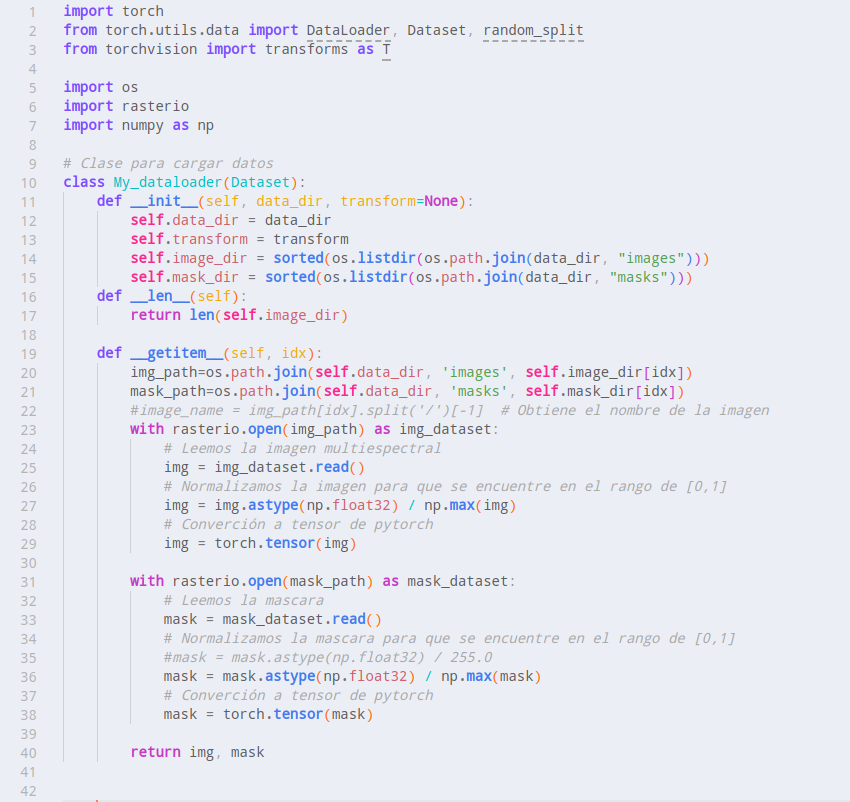
\includegraphics[width=0.98\linewidth]{graficos/cargar_datos}
	%\caption[A]{A}
	%\label{fig:cargar_datos}
\end{figure}

\newpage
\clearpage % Salto de página para separar las secciones
\section*{Anexo B: Código de entrenamiento}

\begin{figure}[h!]
	\centering
	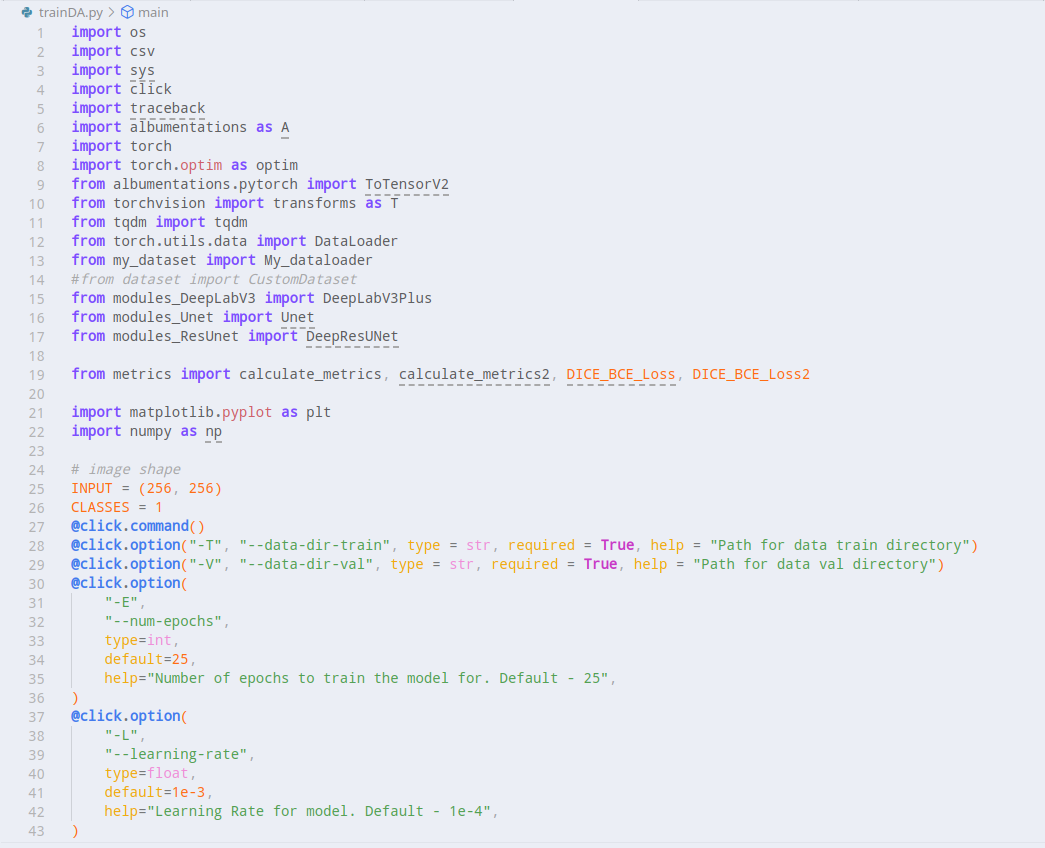
\includegraphics[width=0.9\linewidth]{graficos/entrenamiento}
	%\caption[A]{A}
	%\label{fig:cargar_datos}
\end{figure}

\begin{figure}[h!]
	\centering
	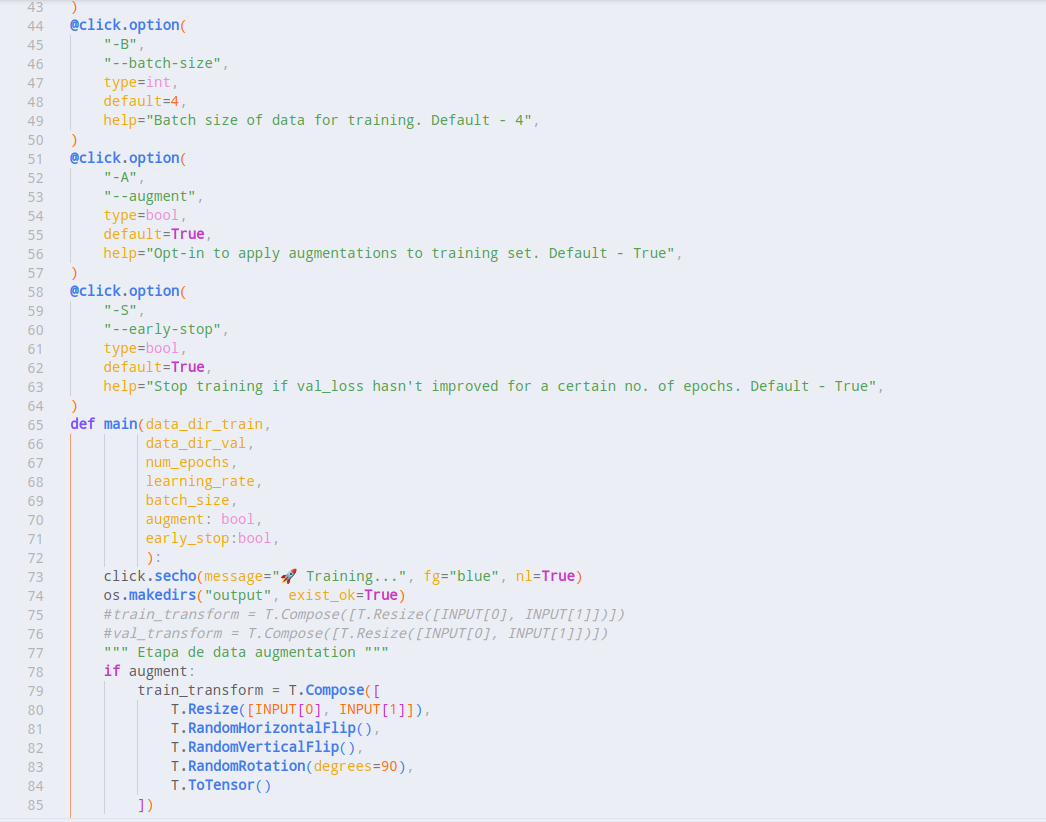
\includegraphics[width=0.9\linewidth]{graficos/entrenamiento2}
	%\caption[A]{A}
	%\label{fig:cargar_datos}
\end{figure}

\begin{figure}[h!]
	\centering
	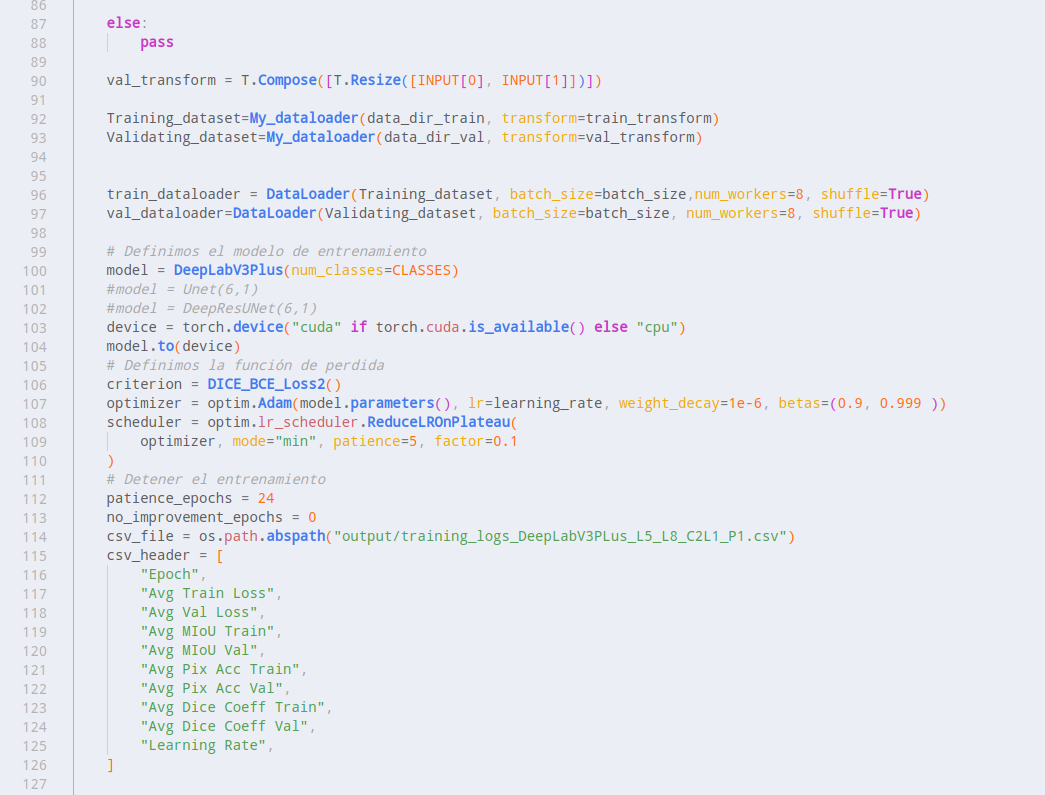
\includegraphics[width=0.9\linewidth]{graficos/entrenamiento3}
	%\caption[A]{A}
	%\label{fig:cargar_datos}
\end{figure}

\begin{figure}[h!]
	\centering
	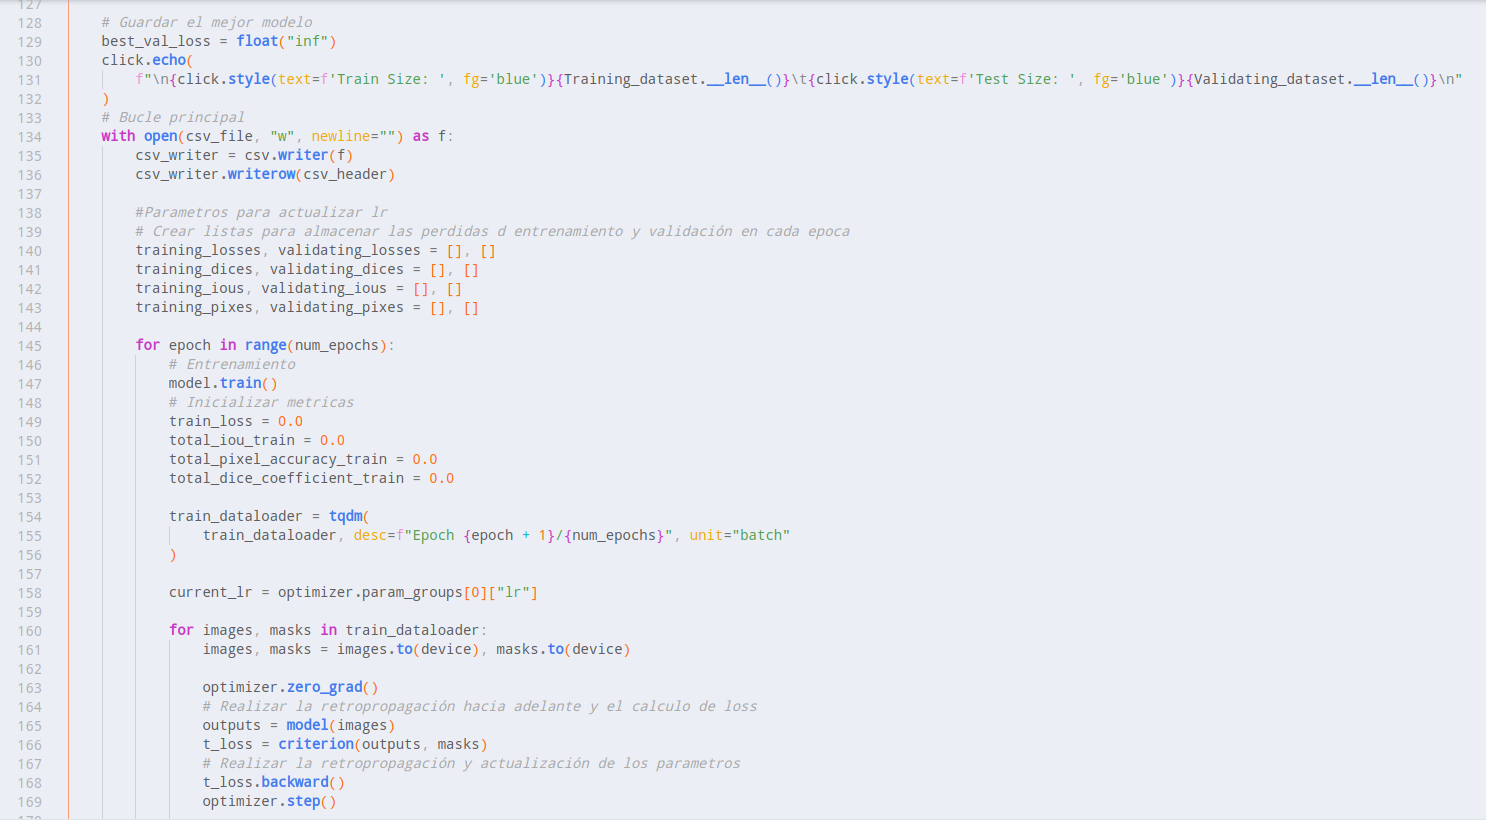
\includegraphics[width=0.9\linewidth]{graficos/entrenamiento4}
	%\caption[A]{A}
	%\label{fig:cargar_datos}
\end{figure}

\begin{figure}[h!]
	\centering
	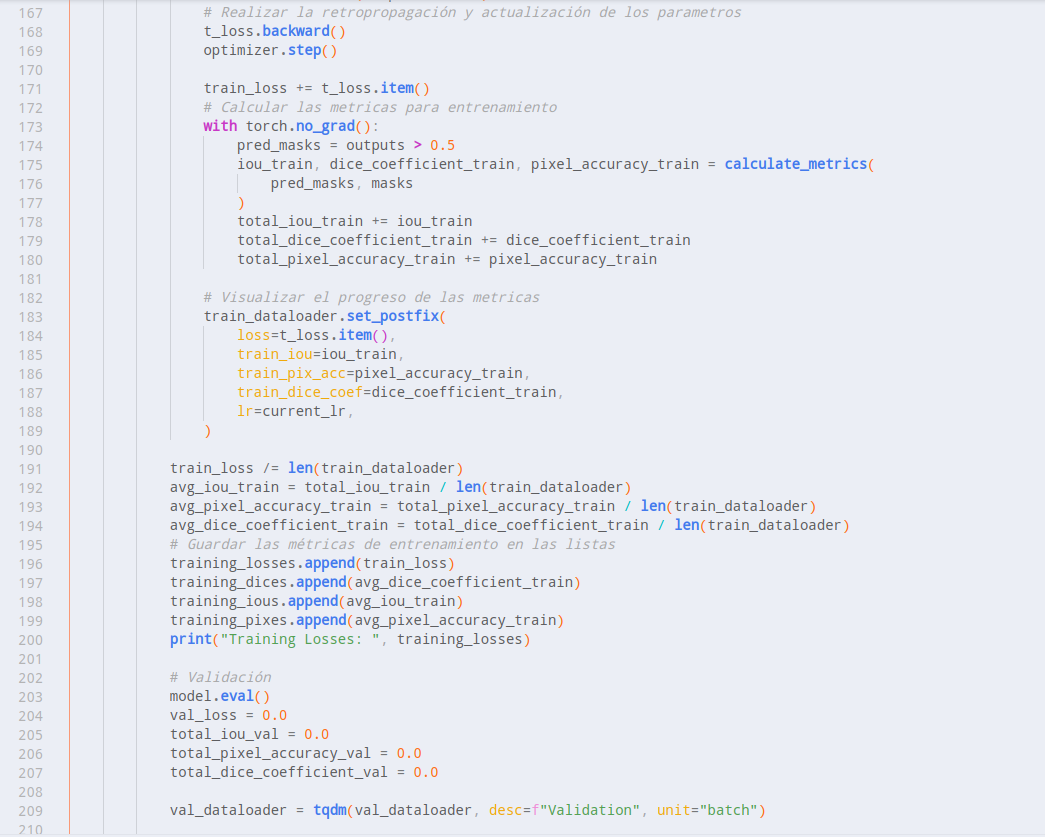
\includegraphics[width=0.9\linewidth]{graficos/entrenamiento5}
	%\caption[A]{A}
	%\label{fig:cargar_datos}
\end{figure}

\begin{figure}[h!]
	\centering
	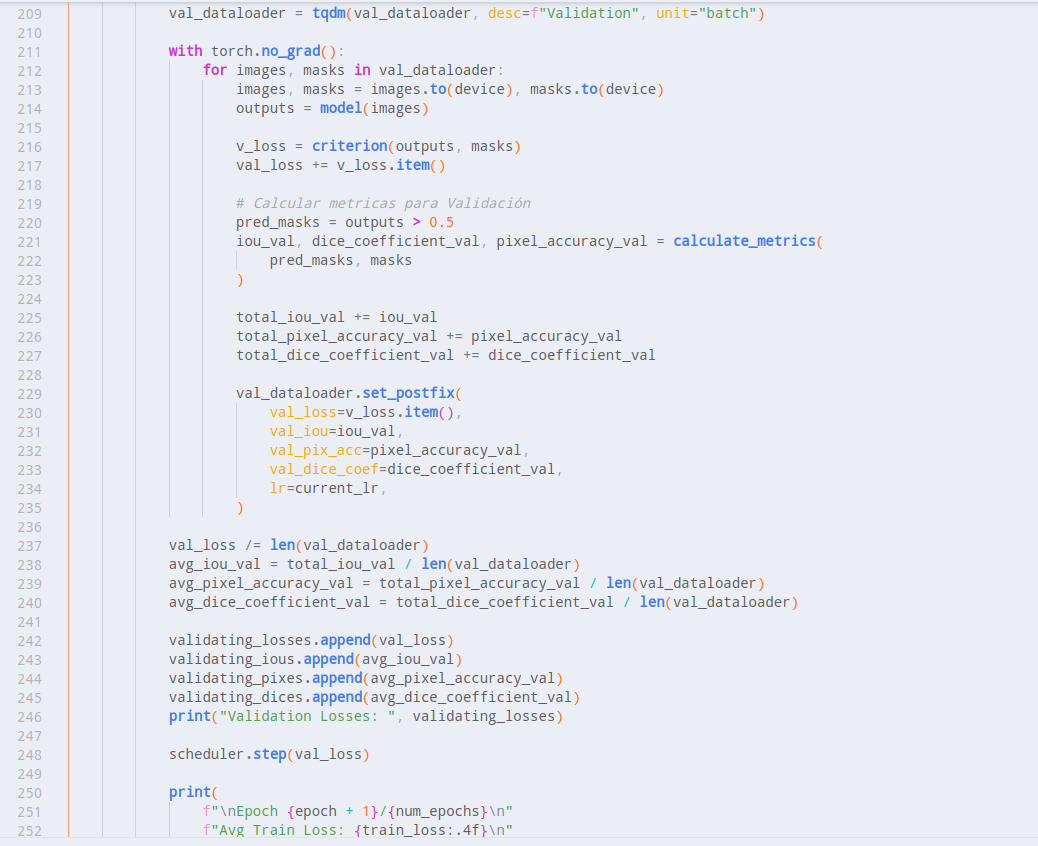
\includegraphics[width=0.9\linewidth]{graficos/entrenamiento6}
	%\caption[A]{A}
	%\label{fig:cargar_datos}
\end{figure}

\begin{figure}[h!]
	\centering
	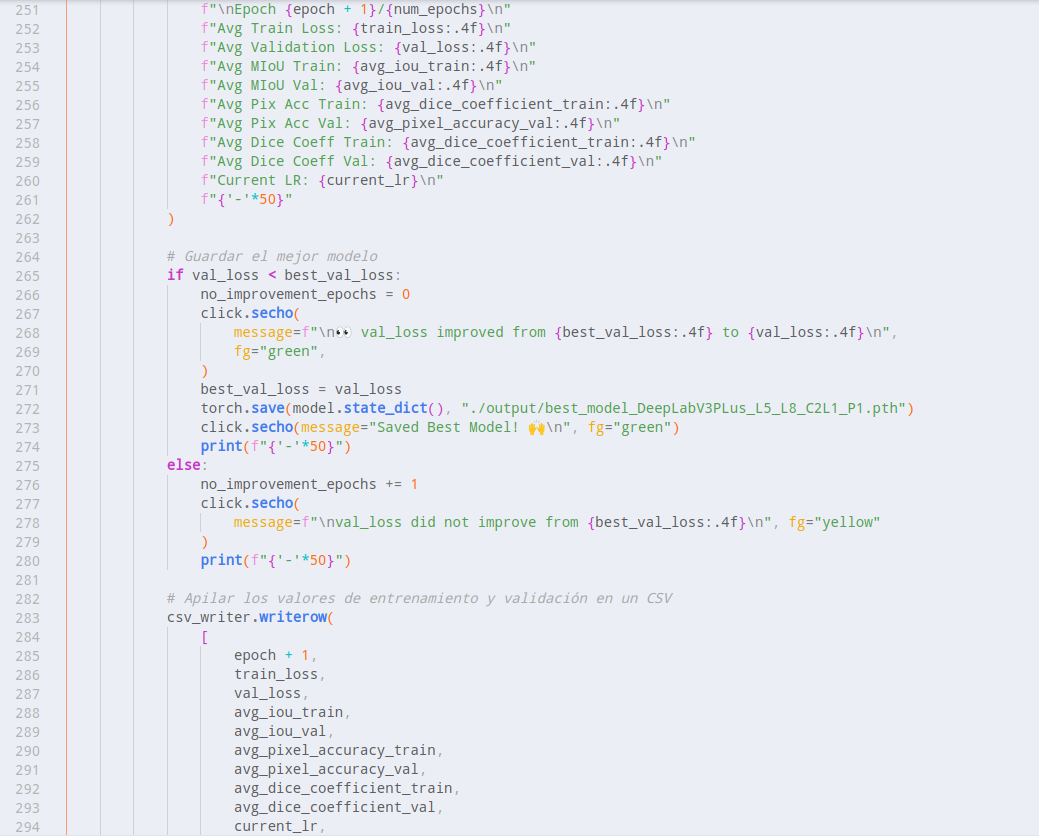
\includegraphics[width=0.9\linewidth]{graficos/entrenamiento7}
	%\caption[A]{A}
	%\label{fig:cargar_datos}
\end{figure}

\begin{figure}[h!]
	\centering
	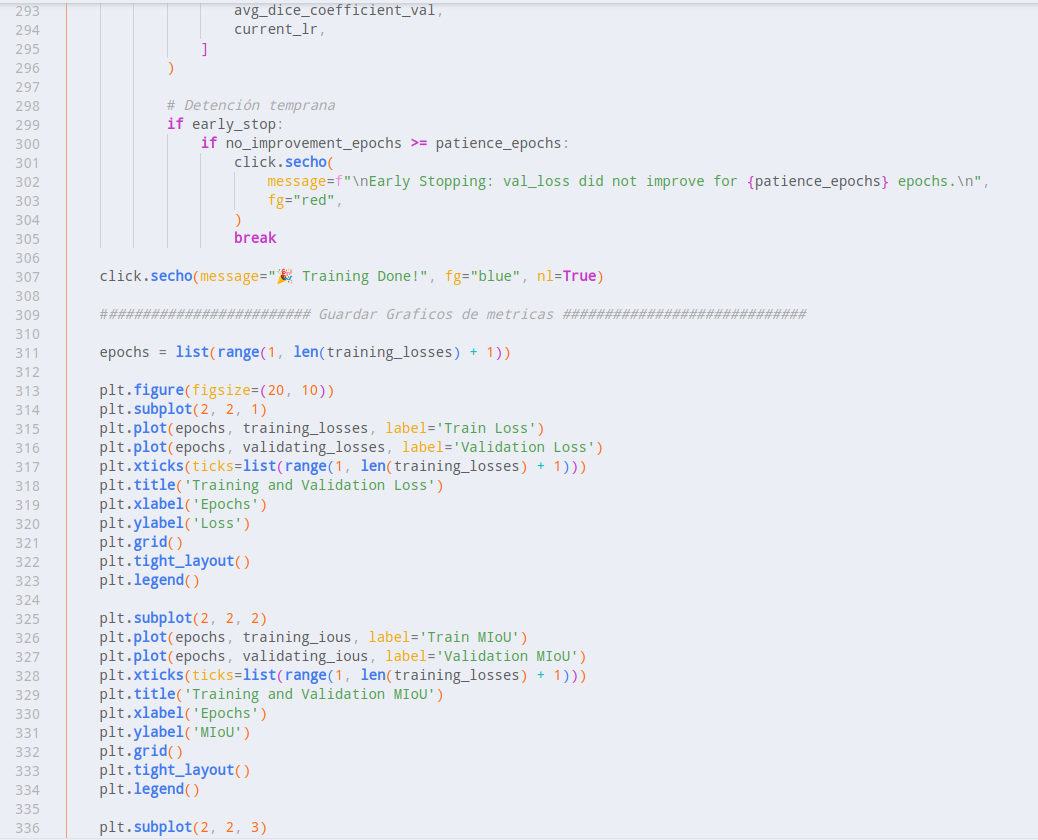
\includegraphics[width=0.9\linewidth]{graficos/entrenamiento8}
	%\caption[A]{A}
	%\label{fig:cargar_datos}
\end{figure}

\begin{figure}[h!]
	\centering
	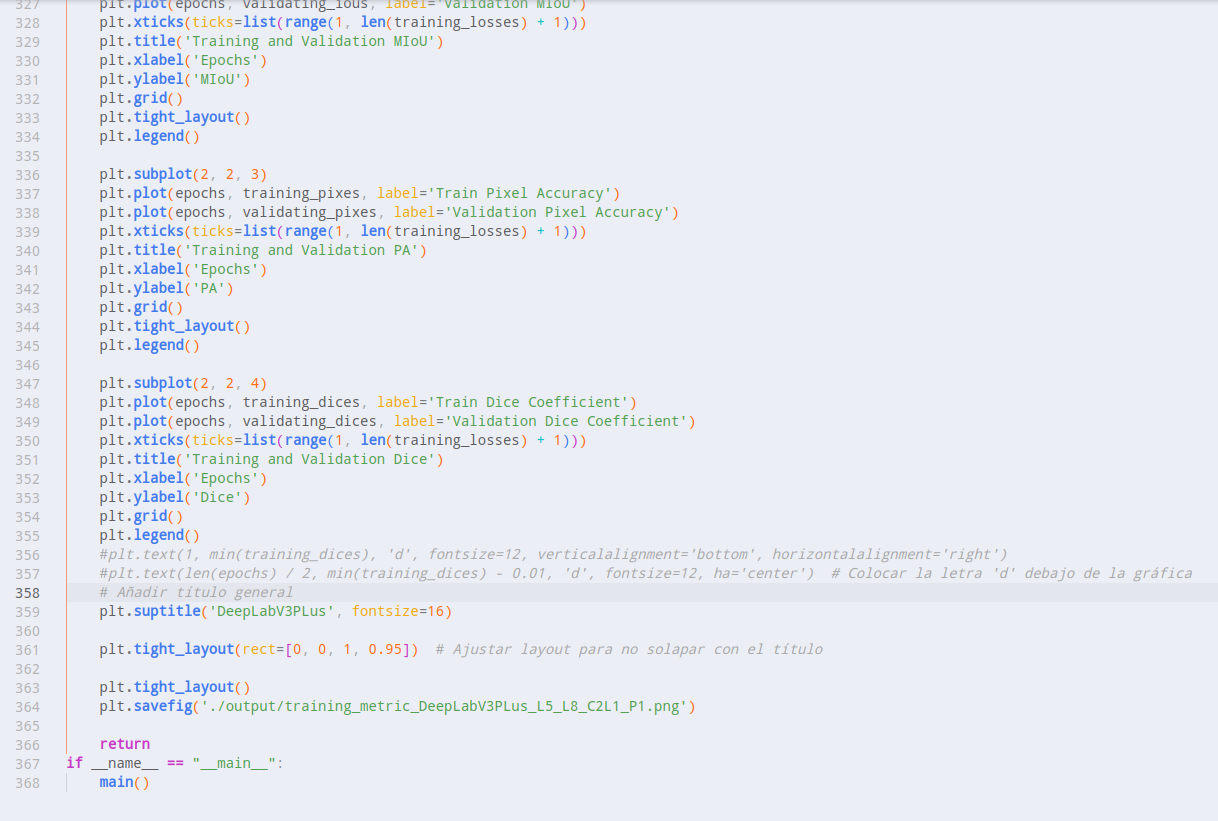
\includegraphics[width=0.9\linewidth]{graficos/entrenamiento9}
	%\caption[A]{A}
	%\label{fig:cargar_datos}
\end{figure}

\newpage
\clearpage % Salto de página para separar las secciones
\section*{Anexo C: Código de evaluación}

\begin{figure}[h!]
	\centering
	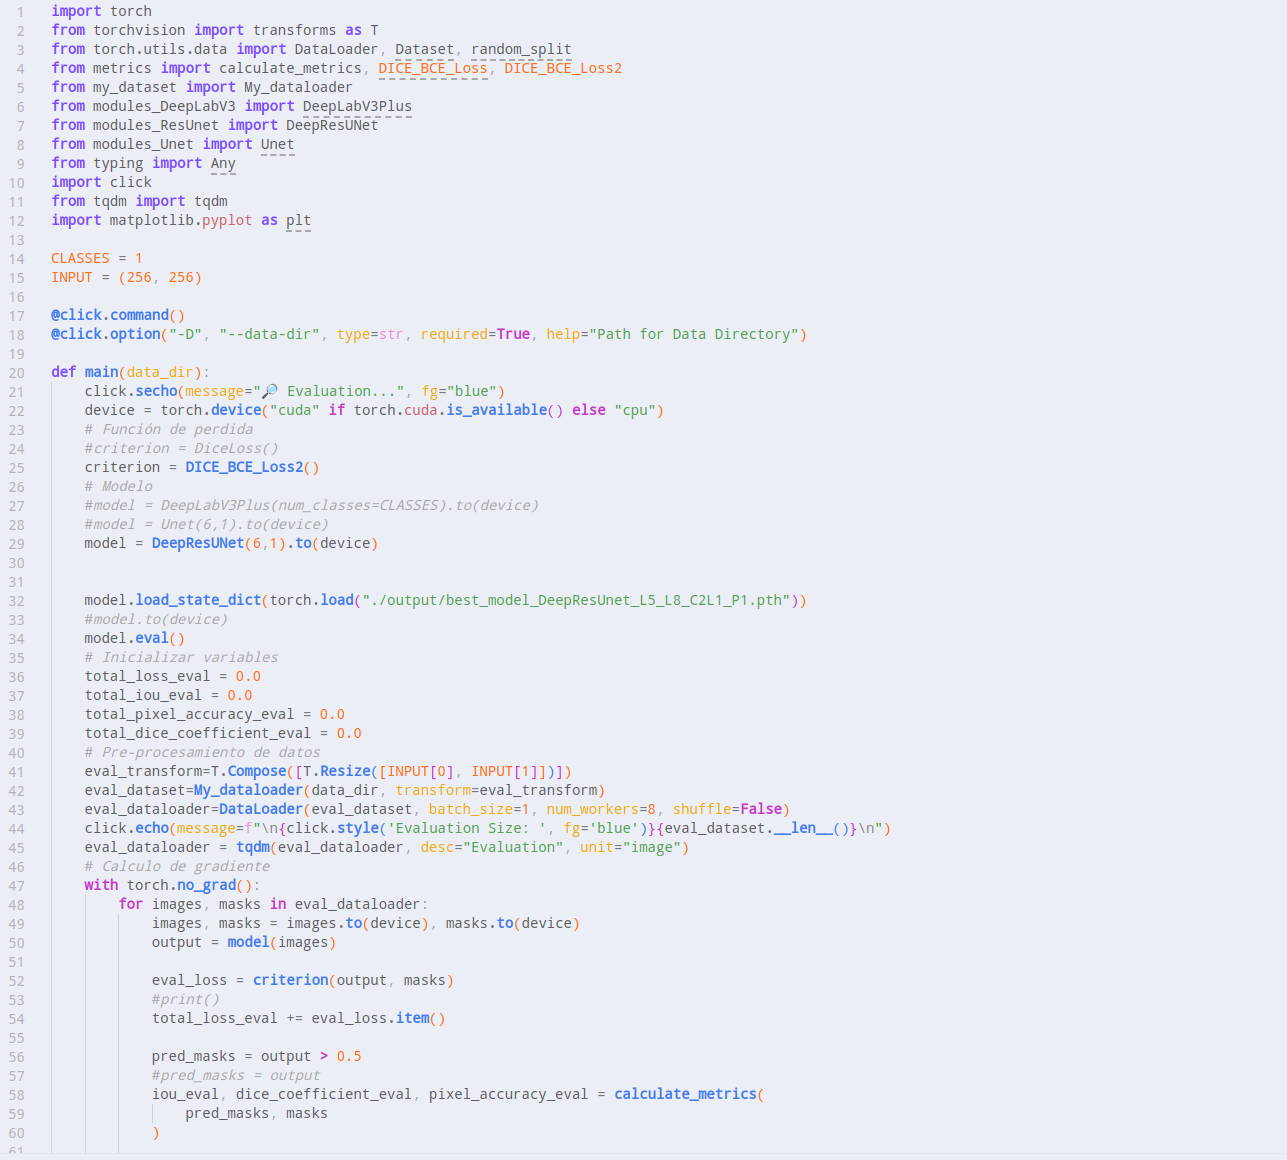
\includegraphics[width=0.9\linewidth]{graficos/test}
	%\caption[A]{A}
	%\label{fig:cargar_datos}
\end{figure}

\begin{figure}[h!]
	\centering
	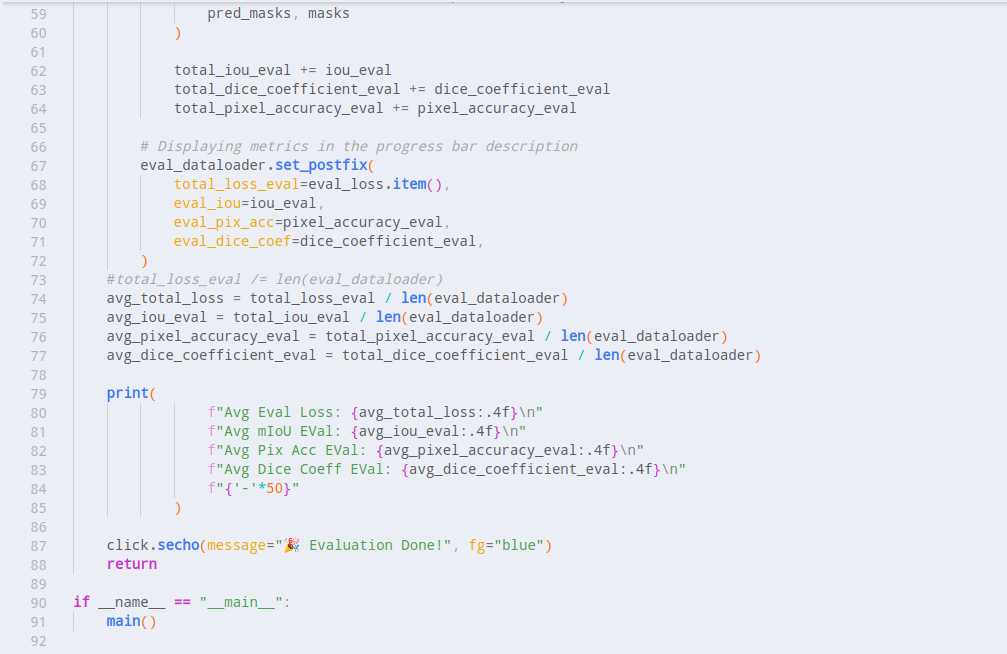
\includegraphics[width=0.9\linewidth]{graficos/test2}
	%\caption[A]{A}
	%\label{fig:cargar_datos}
\end{figure}

\newpage % Salto de página para separar las secciones
\clearpage
\section*{Anexo D: Código Predicción}

\begin{figure}[h!]
	\centering
	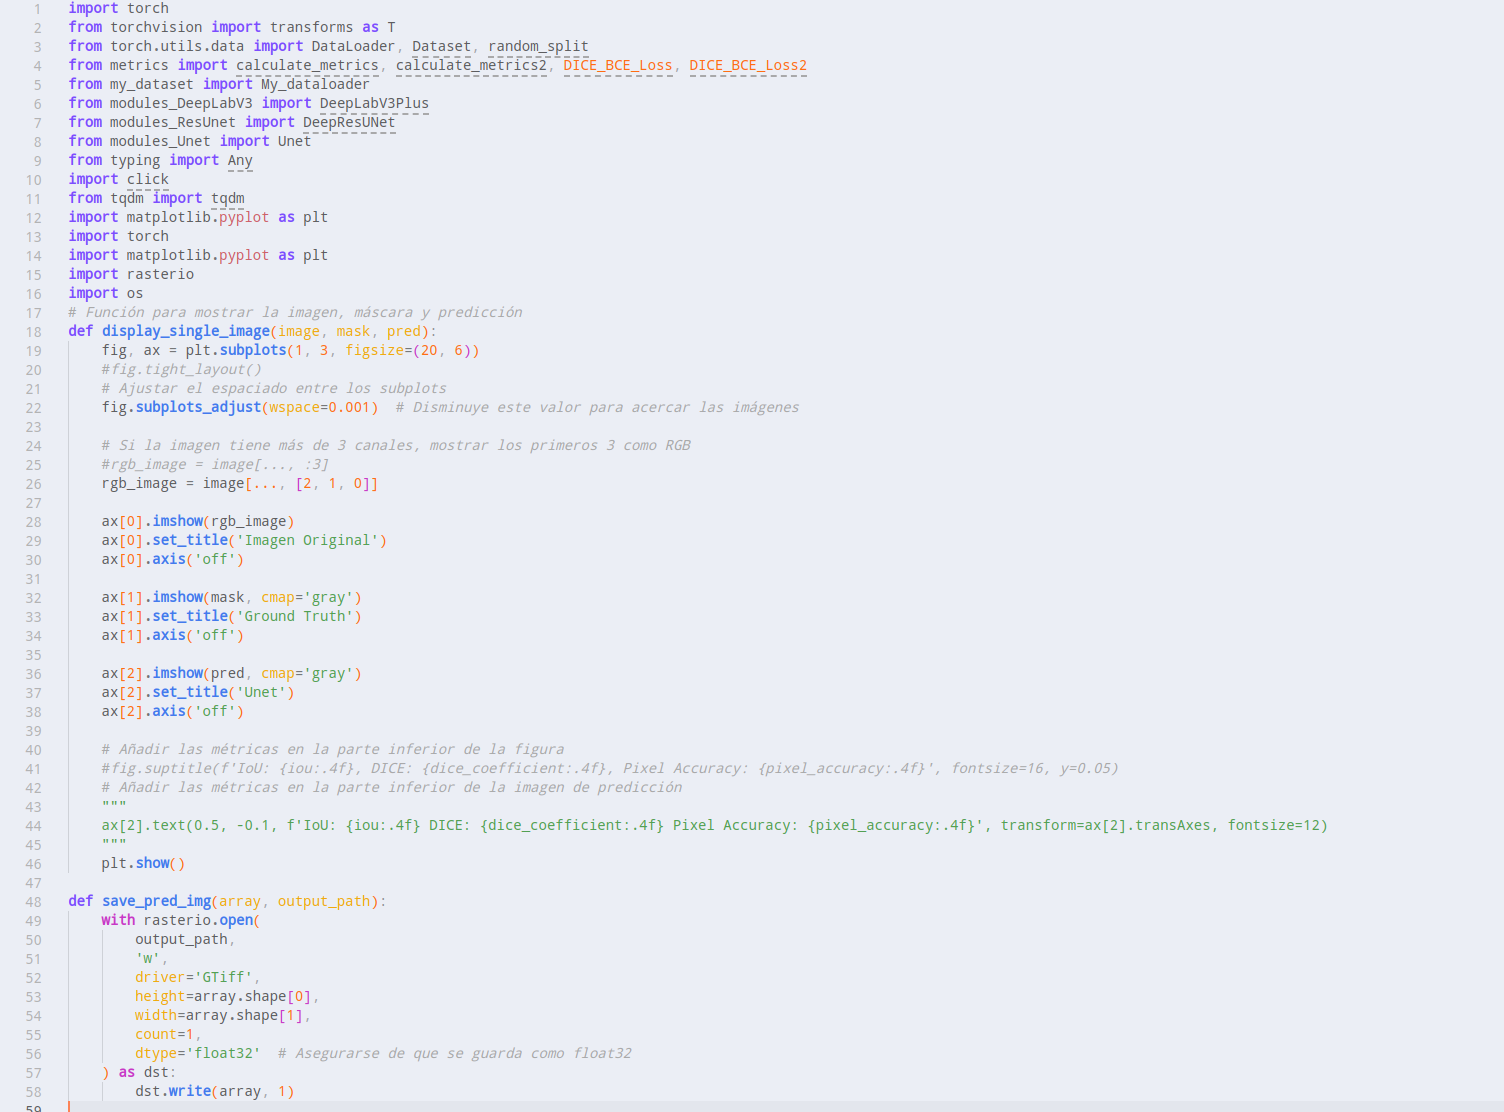
\includegraphics[width=0.9\linewidth]{graficos/pred}
	%\caption[A]{A}
	%\label{fig:cargar_datos}
\end{figure}

\begin{figure}[h!]
	\centering
	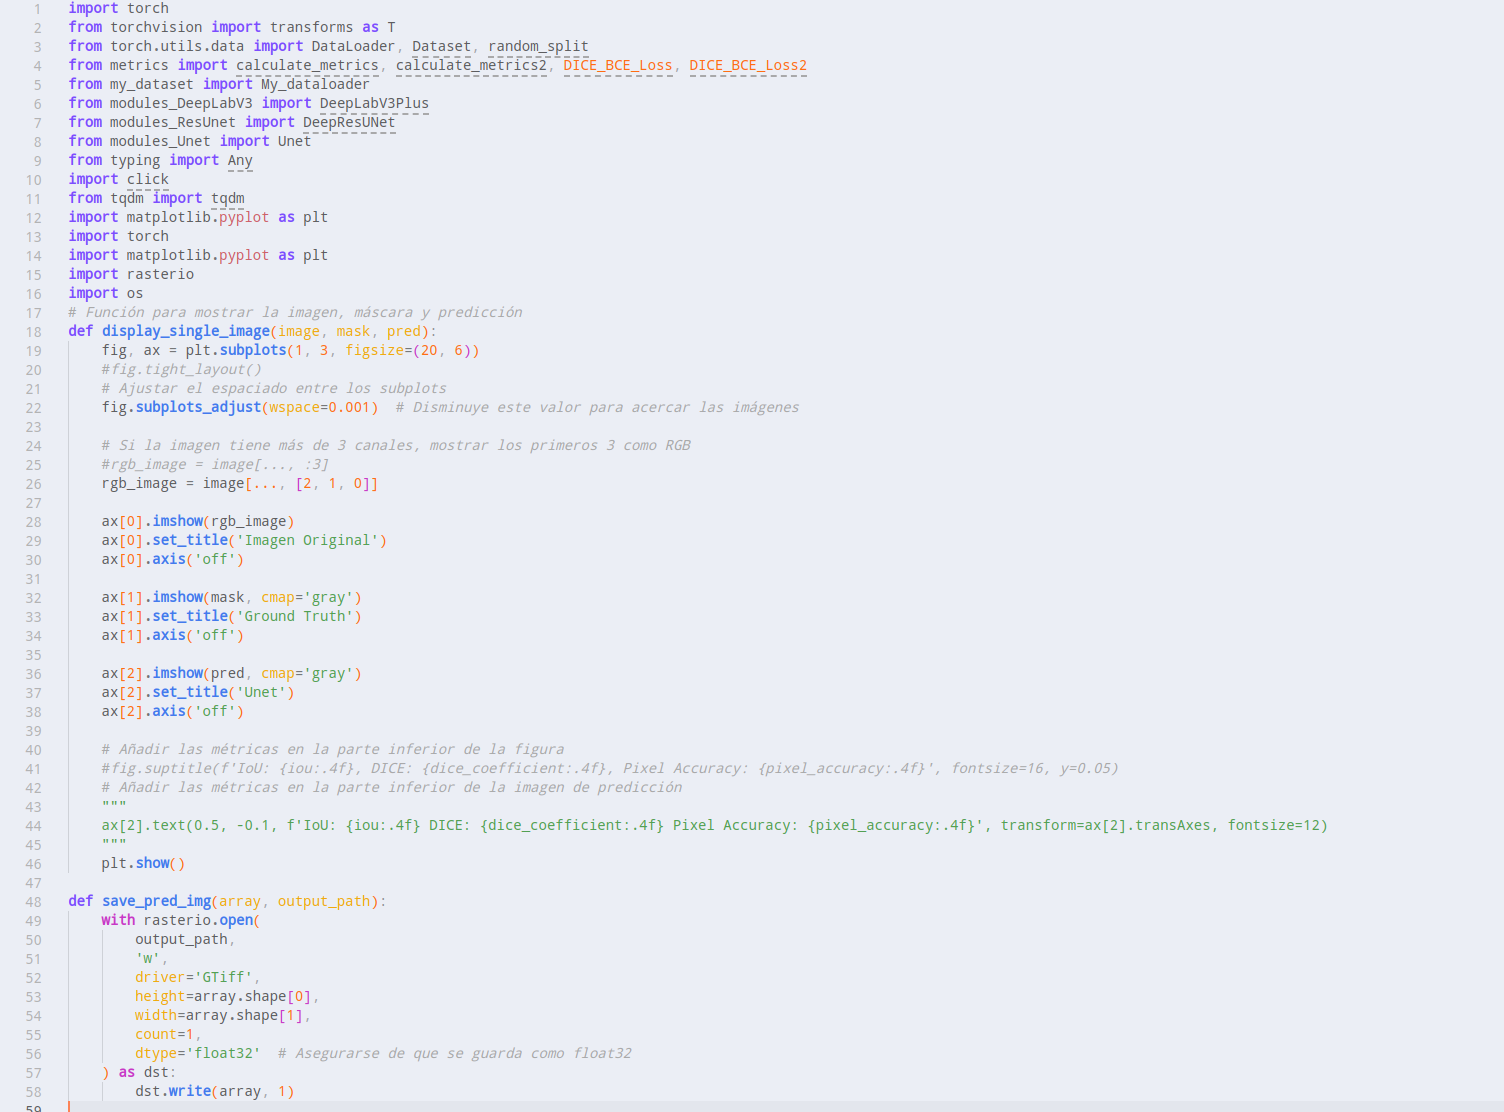
\includegraphics[width=0.9\linewidth]{graficos/pred}
	%\caption[A]{A}
	%\label{fig:cargar_datos}
\end{figure}

\begin{comment}
	\begin{landscape} 
		\pagestyle{empty}
		\chapter*{\begin{center}
				Anexos
		\end{center}}
		\thispagestyle{empty}
		\addcontentsline{toc}{chapter}{Anexos}
		\section*{Anexo A: Diagrama de Gantt}
		
		\begin{table}[h]
			\centering
			\resizebox{\linewidth}{!}{
				\begin{tabular}{m{10cm}|c|c|c|c|c|c|c|c|c|c|c|c|c|c|c|c|c|c|c|c|}
					\hline
					\centering\textbf{Diagrama de Gantt}& \multicolumn{4}{c|}{\centering \textbf{Mes 1}}& \multicolumn{4}{c|}{\centering \textbf{Mes 2}}& \multicolumn{4}{c|}{\centering \textbf{Mes 3}}& \multicolumn{4}{c|}{\centering \textbf{Mes 4}}& \multicolumn{4}{c|}{\centering \textbf{Mes 5}} \\
					\hline
					
					
					\cellcolor{gray!25}Actividad&\cellcolor{gray!25}1&\cellcolor{gray!25}2&\cellcolor{gray!25}3&\cellcolor{gray!25}4&\cellcolor{gray!25}1&\cellcolor{gray!25}2&\cellcolor{gray!25}3&\cellcolor{gray!25}4&\cellcolor{gray!25}1&\cellcolor{gray!25}2&\cellcolor{gray!25}3&\cellcolor{gray!25}4&\cellcolor{gray!25}1&\cellcolor{gray!25}2&\cellcolor{gray!25}3&\cellcolor{gray!25}4&\cellcolor{gray!25}1&\cellcolor{gray!25}2&\cellcolor{gray!25}3&\cellcolor{gray!25}4\\
					
					\hline
					
					Investigar antecedentes de retroceso de glaciar&\cellcolor{blue}&\cellcolor{blue}&\cellcolor{blue}&&&&&&&&&&&&&&&&&\\
					\hline
					Investigar métodos de procesamiento de imágenes de satélite &&&&\cellcolor{blue}&\cellcolor{blue}&&&&&&&&&&&&&&&\\
					\hline
					Descargar y analizar imágenes Landsat 5,7,8 y/o Sentinel-2&&&&&&\cellcolor{blue}&\cellcolor{blue}&&&&&&&&&&&&& \\
					\hline
					Recopilar datasets de la zona de estudio&&&&&&&&\cellcolor{blue}&\cellcolor{blue}&\cellcolor{blue}&&&&&&&&&& \\
					\hline
					Búsqueda de métodos de segmentación&&&&&&&&&&&\cellcolor{blue}&\cellcolor{blue}&&&&&&&& \\
					\hline
					Correcciones necesarias de las imágenes de satelites &&&&&&&&&&&&&\cellcolor{blue}&&&&&&& \\
					\hline
					Procesamiento de imagenes utilizando metodos tradicionales&&&&&&&&&&&&&&\cellcolor{blue}&\cellcolor{blue}&&&&& \\
					\hline
					Implementar el método de segmentación escogido&&&&&&&&&&&&&&&&\cellcolor{blue}&\cellcolor{blue}&&& \\
					\hline
					Obtención de resultados del análisis&&&&&&&&&&&&&&&&&&\cellcolor{blue}&\cellcolor{blue}&\cellcolor{blue}\\
					\hline
					
					
			\end{tabular}}
			%\caption[Sistemas embebidos propuestos]{Sistemas embebidos propuestos.}
			\label{tab:anexoA}
		\end{table}
		\vfill
		\raisebox{0.5 em}{\makebox[\linewidth]{\thepage}}
	\end{landscape}
	\begin{landscape} 
		\thispagestyle{empty}
		\section*{Anexo B: Matriz de consistencia}
		
		\begin{table}[h]
			\centering
			\resizebox{\linewidth}{!}{
				\begin{tabular}{|m{6cm}|m{6cm}|m{6cm}|m{4cm}|m{6cm}|}
					\hline
					\centering\textbf{Problema}& \multicolumn{1}{c|}{\centering \textbf{Objetivos}}& \multicolumn{1}{c|}{\centering \textbf{Hipótesis}}& \multicolumn{1}{c|}{\centering \textbf{Variables}}& \multicolumn{1}{c|}{\centering \textbf{Metodología}}\\
					\hline
					General& General& General& Independiente& Tipo de investigación\\
					\hline
					¿Cómo desarrollar un sistema basado en algoritmos inteligentes que clasifique y segmente cuerpos glaciares para realizar un análisis del retroceso de superficie glaciar?& Aplicar técnicas de deep learning para la clasificación y segmentación de cuerpos glaciares, para realizar un análisis temporal del retroceso de superficie del glaciar Quelccaya, ubicado en la Cordillera Vilcanota, Perú.& El uso de algoritmos inteligentes basados en deep learning para la segmentación de glaciares permitirá realizar un análisis temporal del retroceso glaciar, esto revelará la magnitud de perdida de superficie glaciar.
					& 
					1. Algoritmos de deep learning.
					
					2. Datos de entrenamiento.
					
					3. Parámetros de entrenamiento.
					
					& El presente estudio se enmarca dentro del ámbito de la investigación científica e investigación aplicada, específicamente en el campo de ingeniería y medio ambiente, puesto que se pretende aplicar técnicas de inteligencia artificial, para abordar un problema específico y práctico con un enfoque en el análisis temporal del retroceso glaciar y su gran impacto en el medio ambiente.\\
					\hline
					Específicos& Específicos& Específicas& Dependiente& Nivel de investigación\\
					\hline
					
					1. ¿Qué tipos de algoritmos inteligentes son los más adecuados para la clasificación y segmentación de cuerpos glaciares?
					
					2. ¿Cómo impacta la falta de disponibilidad de datos confiables en el desarrollo de investigaciones de modelos de inteligencia artificial para la segmentación y clasificación de cuerpos glaciares?
					
					3. ¿Cómo llevar a cabo un análisis del retroceso de la superficie glaciar?
					
					4. ¿Cómo comparar los resultados obtenidos de la superficie glaciar a partir de modelos de inteligencia artificial?
					
					&
					1. Utilizar algoritmos de segmentación semántica basados en deep learning para clasificar y segmentar cuerpos glaciares a partir de imágenes de satélite.
					
					2. Desarrollar una base de datos confiable y accesible de imágenes satelitales etiquetadas con cuerpos glaciares para entrenar y evaluar el modelo para tareas de clasificación y segmentación.
					
					3. Analizar los cambios en la superficie glaciar en intervalos de tiempo, utilizando las imágenes clasificadas y segmentadas por el modelo de deep learning, para cuantificar la superficie de retroceso glaciar.
					
					4. Comparar los resultados de superficie glaciar con datos registrados por artículos científicos o instituciones gubernamentales del Perú.
					
					&
					1. Se espera que los algoritmos de deep learning puedan alcanzar algún nivel de precisión en la clasificación y segmentación de cuerpos glaciares, aunque no se puede asegurar si esta precisión será alta.
					
					2. Con el desarrollo de una base de datos, se espera que el modelo implementado tenga precisión y efectividad para tareas de clasificación y segmentación de cuerpos glaciares, aunque la magnitud de esta precisión y efectividad es incierta.
					
					3. El modelo podría ser capaz de identificar y clasificar cuerpos glaciares a lo largo de diferentes estaciones del año, aunque es incierto si podrá hacerlo correctamente, dadas las posibles variaciones temporales en su apariencia.
					
					4. Es incierto si los resultados de la investigación serán comparables y correlacionados con los datos registrados por artículos científicos o instituciones gubernamentales del Perú.
					
					
					& 
					1. Precisión de la clasificación y segmentación.
					
					2. Cobertura glaciar.
					
					3. Retroceso de la superficie glaciar.
					
					&La presente investigación es un estudio científico debido a su nivel de características.\\
					\hline		
			\end{tabular}}
			%\caption[Sistemas embebidos propuestos]{Sistemas embebidos propuestos.}
			\label{tab:anexoB}
		\end{table}
		\vfill
		\raisebox{0.5 em}{\makebox[\linewidth]{\thepage}}
		
	\end{landscape}
	%\pagestyle{fancy}
	\fancyhf{}
	\renewcommand{\headrulewidth}{0pt} 
	\renewcommand{\footrulewidth}{0pt} 
	\fancyfoot[C]{\thepage}
	\section*{Anexo C: Contenido tentativo de la tesis}
	INTRODUCCIÓN
	
	RESUMEN
	
	ABSTRACT
	
	CAPÍTULO 1: GENERALIDADES
	
	1.1 Planteamiento del problema
	
	1.1.1 Problema general
	
	1.1.2 Problemas específicos
	
	1.2 Justificación de la investigación
	
	1.3 Objetivos
	
	1.3.1 Objetivo general
	
	1.3.2 Objetivos específicos
	
	1.4 Variables
	
	1.4.1 Variable Independiente
	
	1.4.2 Variable dependiente
	
	1.5 Metodología
	
	1.6 Alcances
	
	1.7 Limitaciones
	
	CAPÍTULO II: MARCO TEÓRICO
	
	2.1 Antecedentes
	
	2.2 Bases teóricas
	
	2.3 Hipótesis
	
	CAPÍTULO III: METODOLOGÍA
	
	3.1 Estudio y selección de los instrumentos
	
	3.2 Procesamiento del conjunto de datos
	
	3.3 Entrenamiento del conjunto de datos mediante CNN
	
	3.4 Comparación de modelos.
	
	
	CAPÍTULO IV: PRUEBAS Y RESULTADOS
	
	4.1 Prueba de la eficiencia del modelo implementado
	
	CAPÍTULO V: DISCUCIÓN
	
	CAPÍTULO VI: CONCLUSIONES
	
	CAPÍTULO VII: RECOMENDACIONES
	
	REFERENCIAS
	
	ANEXOS
	contenidos...
\end{comment}



